\documentclass[]{article}
\usepackage[english]{babel}
\usepackage{amsmath}
\usepackage{graphicx}
\usepackage[hypcap=false]{caption}
\usepackage{subcaption}
\graphicspath{ {./images/} }
\usepackage{hyperref}
\hypersetup{
	hidelinks
	}

\title{Artificial Intelligence in Cybersecurity: Assignment 3}
\author{Brandon Hosley}
\date{\today}

\begin{document}
	\maketitle
	
\section{Introduction}

In this article \cite{Ballesteros2021} Ballesteros et al. develop a framework that is intended to differentiate between real and fake voice recordings. 
To produce fake voice recordings the team utilizes DeepVoice3 \cite{Ping2018}.
The team bases their work on the outcome of testing three hypotheses.
\begin{description}
	\item[Hypothesis 1] 
		Natural speech signals have very similar statistics to each other, as do fake signals. Additionally, the statistic values between natural and fake signals are dissimilar.
	\item[Hypothesis 2]
		Natural speech signals have very similar entropy values to each other, as do fake signals. Additionally, the entropy values between natural and fake signals are dissimilar.
	\item[Hypothesis 3] 
		Natural speech signals have very similar histogram shapes to each other, as do fake signals. Additionally, the histogram shapes between natural and fake signals are dissimilar.
\end{description}

\section{Data Sources}

% Describe the data used in this paper including source, sample, attribute, etc. (10 points)
To test their hypotheses the team develops several datasets; 100 real and fake for hypothesis 1 and 360 of each for hypothesis 2. 
The 360 real recordings are produced from 44 different speakers who used 4 different languages.
The team makes a sample of their dataset available at this link: \\
\href{https://doi.org/10.17632/ytkv9w92t6.1}{https://doi.org/10.17632/ytkv9w92t6.1}
They then augment the original voice recordings with white noise to double their real dataset.
From each of the 720 real recordings they produce a fake sample.

\section{Algorithm}

% Explain the algorithm/method for visualization in detail from your understanding (20 points)
The Deep4SNet framework works in two parts.
The first part is to convert the audio recording into an image.
For this the research team utilizes the ImageDataGenerator module from Keras.
With this package they convert the file to an image, resize the image, scale it, and flip it horizontally.

In the second part the voice recording images are given to a Convolutional Neural Network (CNN). 
The CNN is trained using a binary-crossentropy loss function.

\begin{equation}
	L(y,\hat{y}) = - \frac{1}{N} \sum_{N}^{i=0} y_i \cdot log(\hat{y}_i) + 
	\langle(1-y_i) \cdot log(1-\hat{y}_i) \rangle
\end{equation}

The activation functions for the convolutional layers and the pooling layers are ReLU.
The output layer has a sigmoid activation function.

\begin{equation}
	f(x) = \frac{1}{1+e^{-x}}
\end{equation}

The CNN structure is visualized below.

% Draw a flowchart of the algorithm for visualization (10 points)
\begin{figure}[h]
	\centering
	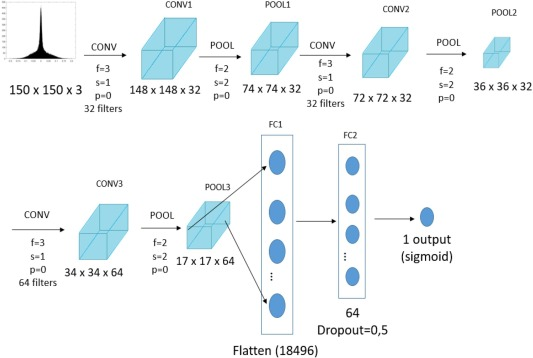
\includegraphics[width=\textwidth]{CNN}
	\caption{Deep4SNet \cite{Ballesteros2021}}
\end{figure}


\section{Results}

% Explain the experimental results in detail from your understanding (10 points)
When tested on their dataset the research team was able to achieve a classification accuracy of 98.5\%.
Deep4SNet was able to achieve precision and recall values aboce 0.9 in all cases except one.
The weakest performance by their model was in correctly identifying real voices, with a recall of 0.814.
This result may be concerning and may not be strong enough for one of their example use cases;
legal proceedings in which the authenticity of a recording has come into question.

\section{Advantages and Disadvantages}

% Discuss the advantages from your understanding (10 points)
This framework achieves very good results with a relatively plain CNN, 
which the authors credit to the pre-processing of recordings into the voice-image histograms that they feed to the neural network.
It is argued that a visual approach optimizes a this type of problem to the strengths of a CNN model.

% Discuss the disadvantages from your understanding (15 points)
The primary disadvantage for this implementation is that it was built on examples exclusively generated through DeepVoice.
While the results prove that the model is very adept at identifying fakes by DeepVoice, 
this does not necessarily prove that the model will work well on fakes generated by other methods.
While it is probable that this framework can be trained on other models as well, 
it is similarly probable that versions of Deep4SNet will be fit to those models.

\section{Improvements}

% Provide the specific ideas to improve the algorithm. General ideas are not allowed. (15 points)
The team approaches their hypotheses and tests them on the basis of data generated from DeepVoice.
While the conclusions may be true for other types of audio fakes, it would be better if the team had tested others as well.
Similarly the testing of Deep4SNet is limited to DeepVoice and would be improved by testing other generative models.

To further this the team would improve the viability of their model against novel generative models if either:
A$)$ theirs were an ensemble trained against different generative models or 
B$)$ the model they trained was based on a dataset comprised of multiple sourced fake samples.

\clearpage
\bibliographystyle{acm}
\bibliography{\jobname}
\end{document}